\documentclass[12pt]{article}
\usepackage{wkrpt}
\begin{document}


\title{Backing Database System for a Messaging Platform Startup}
{
	Ten Thousand Coffees\\
	Toronto, ON
}
{
	Clement Hoang\\
	2B Software Engineering\\
	20531116\\
	c8hoang\\
	May 4th, 2015
}


\letter{Backing Database System for a Messaging Platform Startup}{2A}{Ten Thousand Coffees}{Software Engineering}
{
	\noindent
	Clement Hoang\\
	333 King Street North\\
	Waterloo, ON. 2Z1 N2J
}
{
	Ten Thousand Coffees is startup whose main product is a social networking platform directed towards connecting students with industry professionals. Employed as a member of the core development team for Ten Thousand Coffees, I worked on improving the site and starting experiments over the course of the term. One of the tasks that I was entrusted with was the addition of messaging functionality to Ten Thousand Coffee's online platform.
}
{
	From the the initial planning phase of the messaging system until now, there were several changes of requirements, as well as a limited budget for development. One of the fundamental decisions to make during planning phase was the database system to utilizes for this project. This report analyzes two database systems suitable for backing the messaging platform, and identifies the more appropriate alternative for the project.
}
{
	I would like to thank my co-workers at Ten Thousand Coffees for their continuous guidance during my stay with them. Additionally, I would like to especially thank Elliott Garcea, the lead engineer at Ten Thousand Coffees, for his detailed discussion about our platform's design decisions with me. Finally, I would like to thank my friend, Raymond Wan, for answering a lot of questions that I have about relational database management systems.
}
{
	Clement Hoang, 20531116
}


\tocsection{Executive Summary}
blah blah
The Executive Summary is a one-page summary of the report's highlights, including the purpose and scope of the report, the major points in the report, highlights of the conclusions, and highlights of the recommendations. It is self contained, and is meant to be read and understood by someone (e.g., a company executive officer) who is not likely to read the report itself.

- something about startups
- something about mysql and mongodb (background about traditional relational vs non-relational debate, hard to decide without ocntext, both solve different use cases)
- something about how message is modelled

\newpage


\toc
% \lof
% \lot


\pagenumbering{arabic}
\section{Introduction}
For several decades, the amount of technological startups has been growing and exploring a vast amount of business models to meet the needs of an ever-changing market. From dating sites to smart-watches, there is a business for almost every idea imaginable. Upon closer inspection of the aforementioned startups, there are noticeably many web applications which are primarily focused on messaging, or, at the very least, include a messaging component. To enable messaging capabilities in a web application, there needs to be a web-server to act as the communication bridge between different users, a database to persist user and message data onto for later usage, and a user interface to allow different people to interact with the web application and message other users. The database, in particular, is very important because it serves as a central store for writing and retrieving user generated content such as message content, chat history logs, and various other datasets for use by the application; without the database, a messaging application simply ceases to function.

However, this is where the startup aspect of Ten Thousand Coffees comes into play. Ten Thousand Coffees is a web application that enables users on the site to connect with one another and invite other parties for coffee chats. As a growing company striving to survive in a fierce environment, the importance of a flexible, scalable, and affordable solution is paramount. This is because startups are limited in budget, and have the need the for high growth. In order to have be successful, a startup must be efficient in using the resources that it can afford, and make decisions that enable them to scale both quickly, and affordably, so that they could outperform the competition. For the Ten Thousand Coffees platform, many technical decisions were made during the planning phase, and one such decision was to use MongoDB, a new, open-sourced NOSQL database that is based on a document object model that features horizontal scalability as well as a dynamic schema that allows for agile development. MongoDB was chosen over a traditional SQL database such as MySQL. In contrast, SQL databases have been around for much longer than NOSQL databases, and therefore have gained a lot of enterprise users. A SQL database such as MySQL and a NOSQL database such as MongoDB have completely different design principles, and this report will explore why Ten Thousand Coffees chose MongoDB over MySQL.

\section{Background}
As mentioned in the introduction earlier, Ten Thousand Coffees is a social platform whose mission is to connect the youth of today with the leaders of tomorrow over coffee chats. The solution that the company decided on to approach this problem was a web platform that allows the discovery of possible coffee candidates, with a messaging and scheduling system that allows users to first chat online, before setting up a meeting via the platform and meeting up in real life. The team consists of a business team and a development team, of which contain five and seven employees correspondingly. As a startup with a small team and therefore, limited manpower, there were certain requirements that the chosen database would have to meet in order to be feasible for the platform. These requirements include the ability to prototype rapidly, to be able to scale well, and to be easy-to-use, while still meeting the performance standards for a modern web application. In order to meet these requirements, the team unanimously decided on the MEAN stack, which is a fullstack Javascript framework that became popular over the past few years. For more information on how a web application architectured with the MEAN stack works, see Appendix A.

\section{Rapid Prototyping}
The ability to prototype rapidly is critical to a startup because at the early stages of a company, there is no absolute path from beginning to end goal. This means that the requirements will continuously change and adapt based on feedback received from consumers as well as data gathered by analytics. Because of the need to be able to iterate and improve the platform quickly based on changing requirements, the database management system that is used will need to be flexible so that data can quickly and easily be migrated to support the changing requirements. In this section, the abilities of MongoDB and MySQL to meet the requirements of fast prototyping will be explored.

\subsection{Schema Flexibility}
The criterion of ``schema flexibility'' refers to the ability of a database to adapt to the changing of the data schema. This is an important measure when comparing the benefits of each database system for a messaging platform startup because through the lifetime of the application, the requirements will continuously evolve to meet the demands of the consumers, and it is also not uncommon for bugs at the schema design level to be introduced where a database schema change is necessary in order to fix it.

For example, an early prototype of a messaging platform may only support conversations in which one user can message only one other user. Obviously, most dedicated messaging platforms will eventually improve its functionality to support features such as multi-user messaging, but as an early iteration, to be able to message only one other user is sufficient. Another scenario in which a schema change may be necessary is when a boolean flag field needs to be added into the schema to contain additional state knowledge will helps to solve certain bugs. In these cases, the database management system that is used should be able to migrate or adapt data from the schema of an earlier iteration with a schema of a later iteration with relative ease in order to be a good fit for a startup.

\subsubsection{MongoDB}
MongoDB is a NOSQL database that differs from a MySQL database in that it uses dynamic schemas. Consequently, the documents stored in a collection do not need to have a uniform data model. This schema flexibility allows for migration methods that are different from the usual script method, in which a large script is executed against the database to modify the data models all the relevant data stored in the database at once. With MongoDB's dynamic schema, an alternative approach to schema migration, known as ``lazy updating'' or ``schema versioning.'' Lazy updating refers to the method of only updating documents as required, having code that supports both the older schema as well as the newer one. This allows the database to slowly migrate without any downtime or a large change all at once, until the older schema version is eventually deprecated and support is dropped. At Ten Thousand Coffees, I led the migration of the older messaging schema into the new architecture in order to add support for group messaging. For the sake of brevity, the details of the migration are ommitted from this section. See appendix B for the case study.

-talk about dynamic schema
-more flimsy, allows for slow fallback
-talk about why that makes migration easier
-blah blah see appendix B (for brevity, a lot of details have been ommitted. See appendix B for case study.) -migrating the one-to-many relationships is a lot more annoying as it requires table changes etc. (from 1-1 to group chat)
-show schema figures

\subsubsection{MySQL}
MySQL is a SQL-compliant database which forces the user to define a structure in terms of tables and columns before data can be stored in it. As such, it demands a long initial setup time. This rigidness comes with benefits such as being more reliable and being more efficient at complex queries \cite{sql_vs_nosql}. However, while these benefits are great for a more corporate enterprise solution such as banking software, where reliability is more important, they are not as suited for a startup that is focused on a messaging platform. By SQL's nature, it is more complex to set up then MongoDB, and migrations would also require significantly more effort, as the the mathematical structure containing tables and rows would require a more revamping than simplying adding/removing a field in the case of MongoDB. This is not good for a company that needs fast prototyping. The advantages of rapid prototyping far outweigh the advantages of transaction safety in a startup, and moreso in a messaging platform. In the worst case, if MongoDB performance is bad on certain queries, the relevant components can be swapped for something that is more performant such as Redis. Therefore, MongoDB is more suitable than MySQL is terms of schema flexibility.

-a lot of initial setup time
-rigid structure needs to be defined
-talk about tables
-discuss how it is more complex by nature (not good for fast prototyping)
-show schema figures

-mention something about history loss? - to migrate without losing history

\section{Scaling}

In a startup, the ability for a database to scale is very important. As a startup often starts off with a limited budget and a small initial consumer base, their product does not need to support high traffic. However, as the company grows and their amount of users rises, then the ability to support the increased traffic is mandatory in order for the company to survive. Different technologies have different techniques to handle specific use cases and so, the characteristics of different databases will vary when they scale. There is a common theorem known as the ``CAP'' theorem where no system can achieve consistency, high-availability, and partition-tolerance at the same time, and this is made especially apparent when scaling the database management system. A consistent system is one where the system can guarantee that the same state will be reported at all nodes in every subsequent operation until the state is explicitly changed. A system that is highly available is one that is resistant to hardware failure and allows operations to continue even if a node has failed. Finally, a partition-tolerant system is one where the system can be split over several datacenters while staying synchronized with one another. \cite{cap_theorem}

\begin{figure}
\begin{center}
        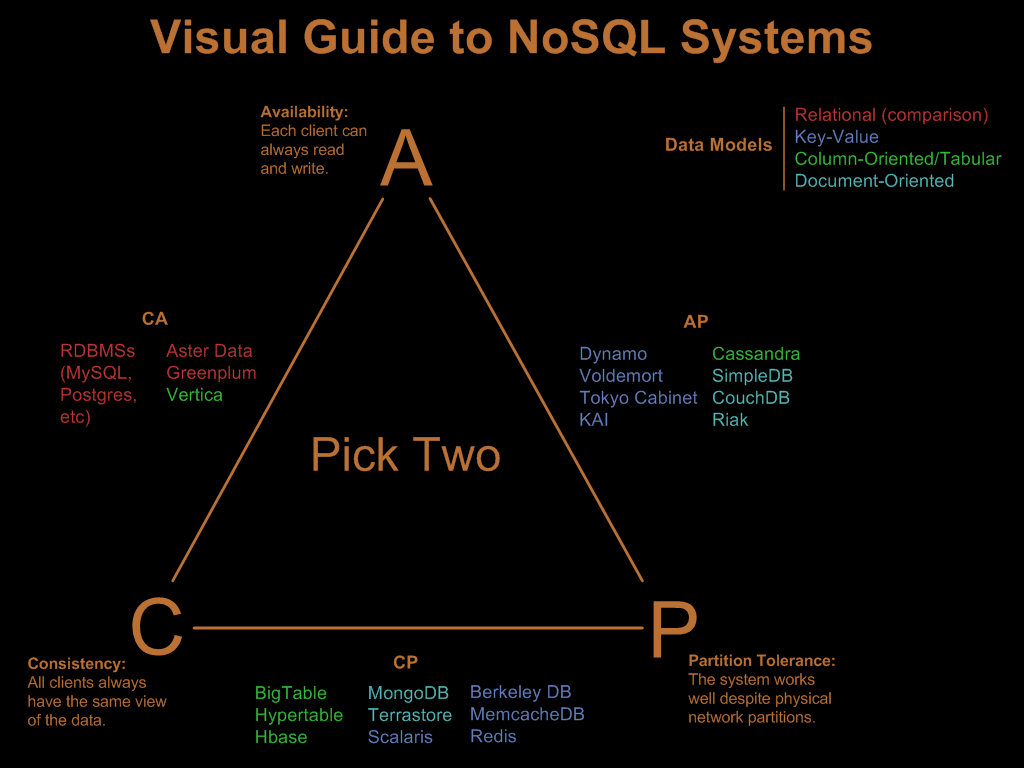
\includegraphics[scale=0.4]{resources/choose_two.png}
\end{center}
\caption{\label{figcaption} A visual representation of Brewer's CAP Theorem \cite{cap_picture}}
\end{figure}

\subsection{MongoDB}
%http://docs.mongodb.org/manual/core/sharding-introduction/
%http://www.mongodb.com/mongodb-scale

In terms of the CAP Theorem, MongoDB has very high partition-tolerance. One of the reasons that it is so popular is because of its ability to horizontally scale very well.

-mention how it horizontally scales
-mention how it can also vertically scale, like sql systems

\subsection{MySQL}
-mention how it can vertically scales
-mention how although it was not made to horizontally scale, it could, with some tools/work
-mention maybe some ways that mysql can horizontally scale, mention that it's not native


-overall mongo wins because it comes with support out of the box

\section{Performance}
The Main Sections of the report are the heart of the report, containing detailed descriptions of the technical decision being reported. In an analysis report, the Main Sections start by elaborating on the problem identified in the Introduction , expanding on the problem definition and on background material relevant to understanding the problem. They describe the analytical study or the experiment performed, and explicate and justify any assumptions made. They conclude by reporting the results of the study, drawing conclusions, and making recommendations. To be complete, an analysis report should identify any threats to the validity of the analysis' results, and should describe the costs and consequences of following, and of not following, the recommendations. In a synthesis report, the Main Sections start by elaborating on the problem identified in the Introduction, expanding on the problem definition to include rigorous and precise specifications of the design criteria and constraints. The sections describe your solution to the problem, including an explanation of how your solution satisfies the design criteria and constraints. They also report alternative designs and solutions that were considered, and they explain why the proposed solution is most favourable in the given context. To be complete, a synthesis report should identify any limitations of the solution proposed.



\section{Conclusions}
CONCLUSIONS
blah blah something results (summarize results and constrast)
it is clear that mongodb matches the criteria better
mysql suited for other purposes...such as complexity or something else, but it is not a good fit in an environment that is continuously changing and evolving
\cite{smpl}

\section{Recommendations}
RECOMMENDATIONS

\newpage


\addcontentsline{toc}{section}{\refname}
\bibliography{wkrpt}
\newpage


\tocsection{Acknowledgements}
ACKNOWLEDGEMENTS
\newpage


\appendix{A}{The MEAN Stack}

The MEAN stack is a fullstack Javascript framework for web applications. It differs from other web frameworks such as Ruby on Rails, or Python with Django in that it is a monoglot framework and only uses Javascript for both its front-end and its backend logic. Because the MEAN stack is fully Javascript, that means most web developers will be able to learn how to program with the MEAN stack with relative ease, as Javascript is virtually the only front-end programming language that exists for web development, and they will have had at least some experience with it.

MEAN is an acronym that stands for MongoDB, Express.js, Angular.js, and Node.js. This section of the appendix will explain each component of the MEAN stack, and how they interact with each other.

MongoDB %(http://docs.mongodb.org/manual/faq/fundamentals/#what-kind-of-database-is-mongodb)
MongoDB is a document-oriented DBMS. Think of MySQL but with JSON-like objects comprising the data model, rather than RDBMS tables. Significantly, MongoDB supports neither joins nor transactions. However, it features secondary indexes, an expressive query language, atomic writes on a per-document level, and fully-consistent reads.
-include the link where it is mapped to SQL?

Express.js %(http://expressjs.com/)
Express is a minimal and flexible Node.js web application framework that provides a robust set of features for web and mobile applications.
It provides a nice interface for Node to route requests to different paths, etc. and has a middleware system blah blah.
-include some express code snippets

Angular.js %(https://docs.angularjs.org/guide/introduction)
AngularJS is a structural framework for dynamic web apps. It lets you use HTML as your template language and lets you extend HTML's syntax to express your application's components clearly and succinctly. Angular's data binding and dependency injection eliminate much of the code you would otherwise have to write. And it all happens within the browser, making it an ideal partner with any server technology.
-include some example of Angular interpolations in html

Node.js %(https://nodejs.org/)
Node.js is a platform built on Chrome's JavaScript runtime for easily building fast, scalable network applications. Node.js uses an event-driven, non-blocking I/O model that makes it lightweight and efficient, perfect for data-intensive real-time applications that run across distributed devices.
-mention some stuff about how it is good with concurrency but not cpu-intensive operations (maybe with reference)
-add a diagram from (http://www.toptal.com/nodejs/why-the-hell-would-i-use-node-js)

With the MEAN architecture, Node with Express is the event-drive server that handles user requests as well as API calls from the client. The user would be interacting with the Angular site that is served statically via the Express server, and their interaction with the site would lead to actions being triggered. These actions will interact with the application's API through HTTP requests. Through the web application's API, updates, retrievals, and posts would be made to the fields in the MongoDB database.

-include diagram here with caption

\newpage

\appendix{B}{Case Study of Schema Migration at Ten Thousand Coffees}
blah blah

\newpage

\end{document}
